\documentclass[a4paper]{tufte-book}

\hypersetup{colorlinks}% uncomment this line if you prefer colored hyperlinks (e.g., for onscreen viewing)

%%
% Book metadata
\title{Process Book}
\author{Data Visualization - Kirell Benzi}
\publisher{Robin Clerc, Kristina Satara, Lara Wietschorke}

%%
% If they're installed, use Bergamo and Chantilly from www.fontsite.com.
% They're clones of Bembo and Gill Sans, respectively.
\IfFileExists{bergamo.sty}{\usepackage[osf]{bergamo}}{}% Bembo
\IfFileExists{chantill.sty}{\usepackage{chantill}}{}% Gill Sans


%\usepackage{microtype}

\usepackage[english]{babel}
\usepackage{comment} % enables the use of multi-line comments (\ifx \fi) 

%%
% For nicely typeset tabular material
\usepackage{booktabs}

%%
% For graphics / images
\usepackage{graphicx}
\setkeys{Gin}{width=\linewidth,totalheight=\textheight,keepaspectratio}
\graphicspath{{graphics/}}

% The fancyvrb package lets us customize the formatting of verbatim
% environments.  We use a slightly smaller font.
\usepackage{fancyvrb}
\fvset{fontsize=\normalsize}

%%
% Prints argument within hanging parentheses (i.e., parentheses that take
% up no horizontal space).  Useful in tabular environments.
\newcommand{\hangp}[1]{\makebox[0pt][r]{(}#1\makebox[0pt][l]{)}}

%%
% Prints an asterisk that takes up no horizontal space.
% Useful in tabular environments.
\newcommand{\hangstar}{\makebox[0pt][l]{*}}

%%
% Prints a trailing space in a smart way.
\usepackage{xspace}

% Prints the month name (e.g., January) and the year (e.g., 2008)
\newcommand{\monthyear}{%
  \ifcase\month\or January\or February\or March\or April\or May\or June\or
  July\or August\or September\or October\or November\or
  December\fi\space\number\year
}

% Inserts a blank page
\newcommand{\blankpage}{\newpage\hbox{}\thispagestyle{empty}\newpage}

\usepackage{units}

% Typesets the font size, leading, and measure in the form of 10/12x26 pc.
\newcommand{\measure}[3]{#1/#2$\times$\unit[#3]{pc}}

% Macros for typesetting the documentation
\newcommand{\hlred}[1]{\textcolor{Maroon}{#1}}% prints in red
\newcommand{\hangleft}[1]{\makebox[0pt][r]{#1}}
\newcommand{\hairsp}{\hspace{1pt}}% hair space
\newcommand{\hquad}{\hskip0.5em\relax}% half quad space
\newcommand{\TODO}{\textcolor{red}{\bf TODO!}\xspace}
\newcommand{\ie}{\textit{i.\hairsp{}e.}\xspace}
\newcommand{\eg}{\textit{e.\hairsp{}g.}\xspace}
\newcommand{\na}{\quad--}% used in tables for N/A cells
\providecommand{\XeLaTeX}{X\lower.5ex\hbox{\kern-0.15em\reflectbox{E}}\kern-0.1em\LaTeX}
%\newcommand{\tXeLaTeX}{\XeLaTeX\index{XeLaTeX@\protect\XeLaTeX}}
% \index{\texttt{\textbackslash xyz}@\hangleft{\texttt{\textbackslash}}\texttt{xyz}}
\newcommand{\tuftebs}{\symbol{'134}}% a backslash in tt type in OT1/T1

\newcommand{\quo}[1]{\flqq{#1}\frqq}


% Generates the index
\usepackage{makeidx}
\makeindex

\begin{document}
% r.3 full title page
\maketitle

% r.5 contents
\tableofcontents
\listoffigures
\listoftables

% Start the main matter (normal chapters)
\mainmatter


\chapter{Finding the Perfect Idea}
\label{ch:idea}

\newthought{The first step} we took was brainstorming. After the announcement of the project we collected several ideas. Finally we choose the idea of football player transfers, which we will explain in detail in the following section.

\section{Football Player Transfers}
Inspired by famous games like the FIFA series and Football Manager, we want to visualize the transfers of professional football players all over the world, but also visualize data about the players and clubs themselves. For these games there was already a lot of data collected, but it was only used for the gameplay. Unfortunately it's not possible to explore the data within these games. \\
Our motivation is to make this data available to the many people all over the world which are not only interested in football game statistics, but also in an overview of the transfer flow of players. The teams are always in change and there are a lot of transfers made in this business. It's hard to keep every transfer in mind to have an overview. And the people who were observing this business for some years usually develop the feeling, that young players come to Europe to play in the famous leagues while they leave to Asia and Northern America when the players become older. But is this really true? If so, what are the possible reasons? Are the performances of players in leagues from different continents really that different as it seems to us? And do clubs maybe have a typical transfer strategy? If we match the transfer data with additional information of the player, can we maybe discover more about the transfer? Does the money used to buy a new player always depend on his last performances? Or are there also other factors? There are a lot of questions and hopefully our visualization will bring us a bit closer to an explanation. The target audience is on the one hand young people interested in football players and clubs. For them 
we will create a search function to make exactly the data accessible they are looking for. On the other hand we want to give people who are new to that topic the possibility to discover it with predefined filters. \\
In fact we wanted to visualize the transfers with curves on a world map, using different colors to encode the age. By using several filters we could e.g. also use the color to encode the transfer sum. We wanted to give the user the possibility to search for a player or a club and by this only visualize the transfers of this player (the color encodes the chronology of his transfers) or the club. \\
By clicking on the name and picture/logo, we would extend an overlay with additional information like a brief curriculum vitae of the player and a brief information part about his current club. Also we could show a list of players, with whom the selected player has played in another club before.

\begin{figure}
  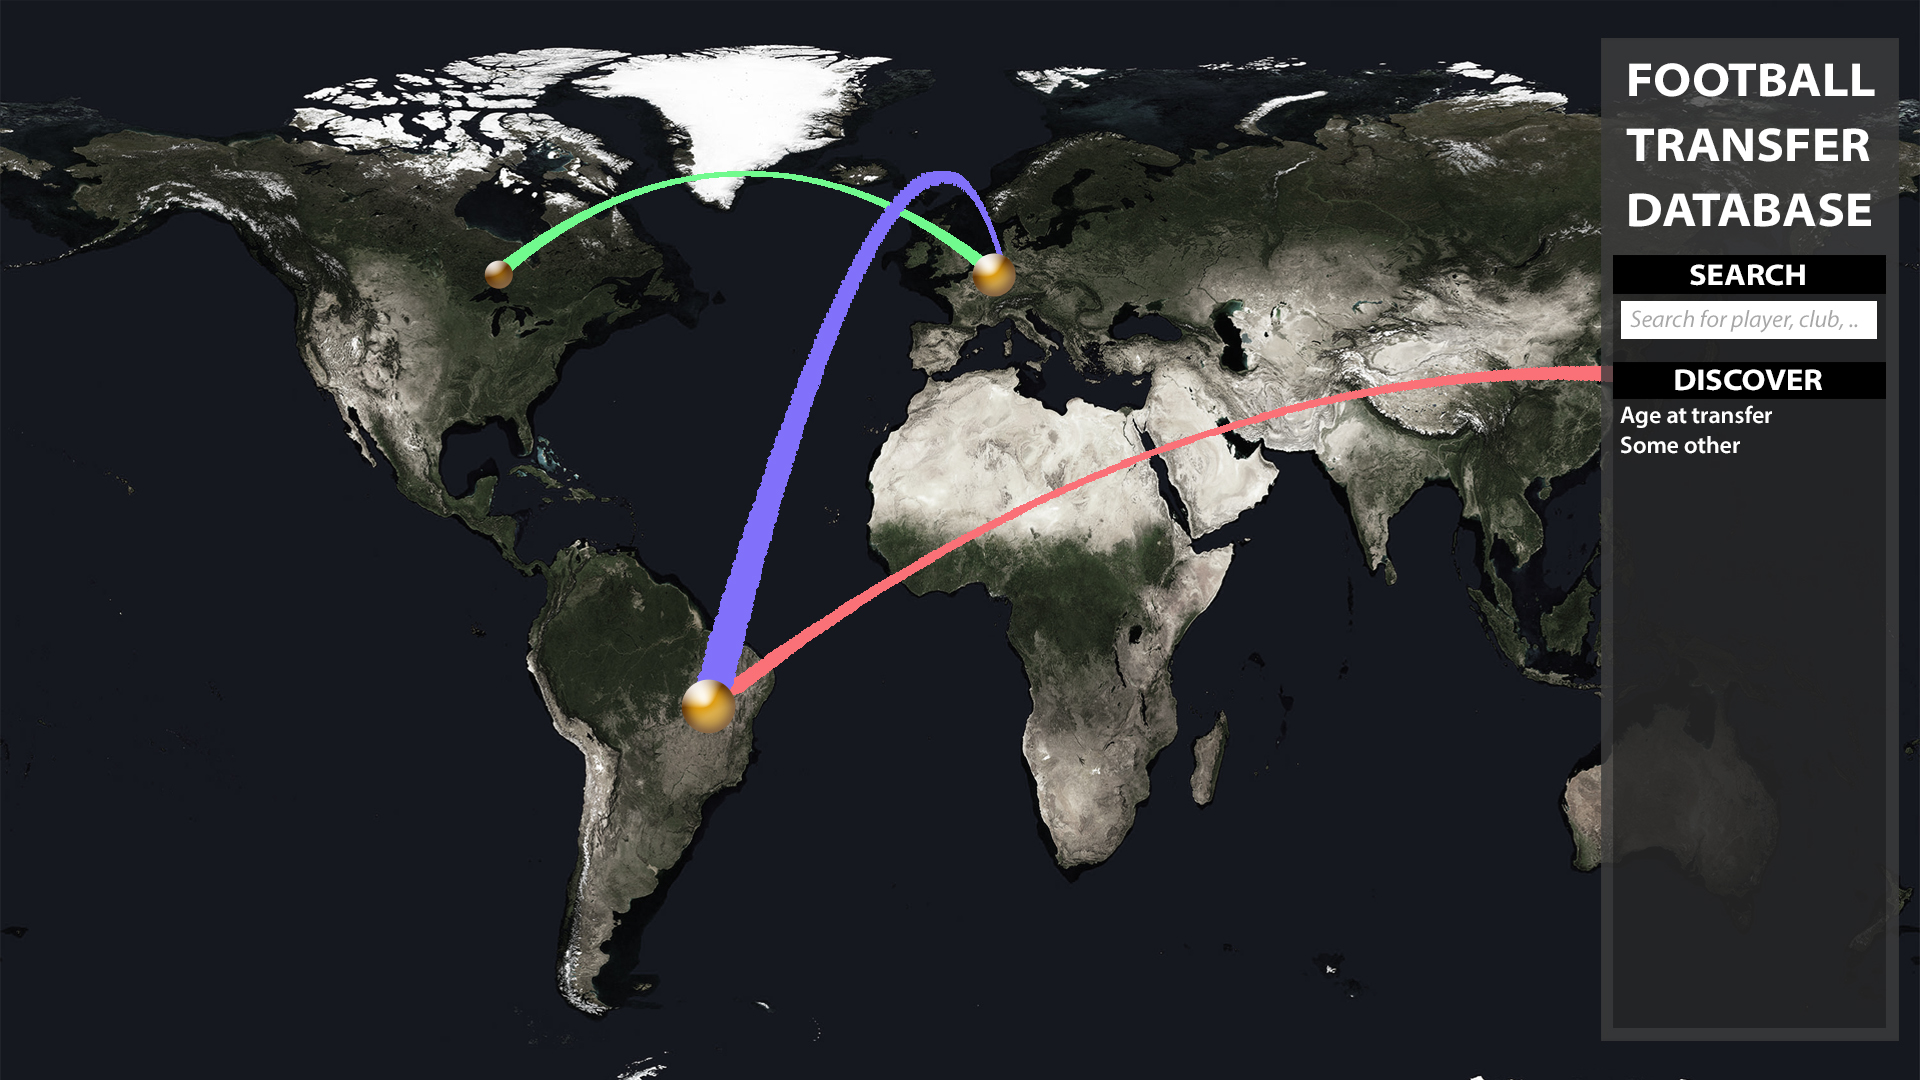
\includegraphics{Images/general_map.jpg}%
  \caption{Mockup of the map, when entering the visualization.}%
\end{figure}

\begin{figure}
  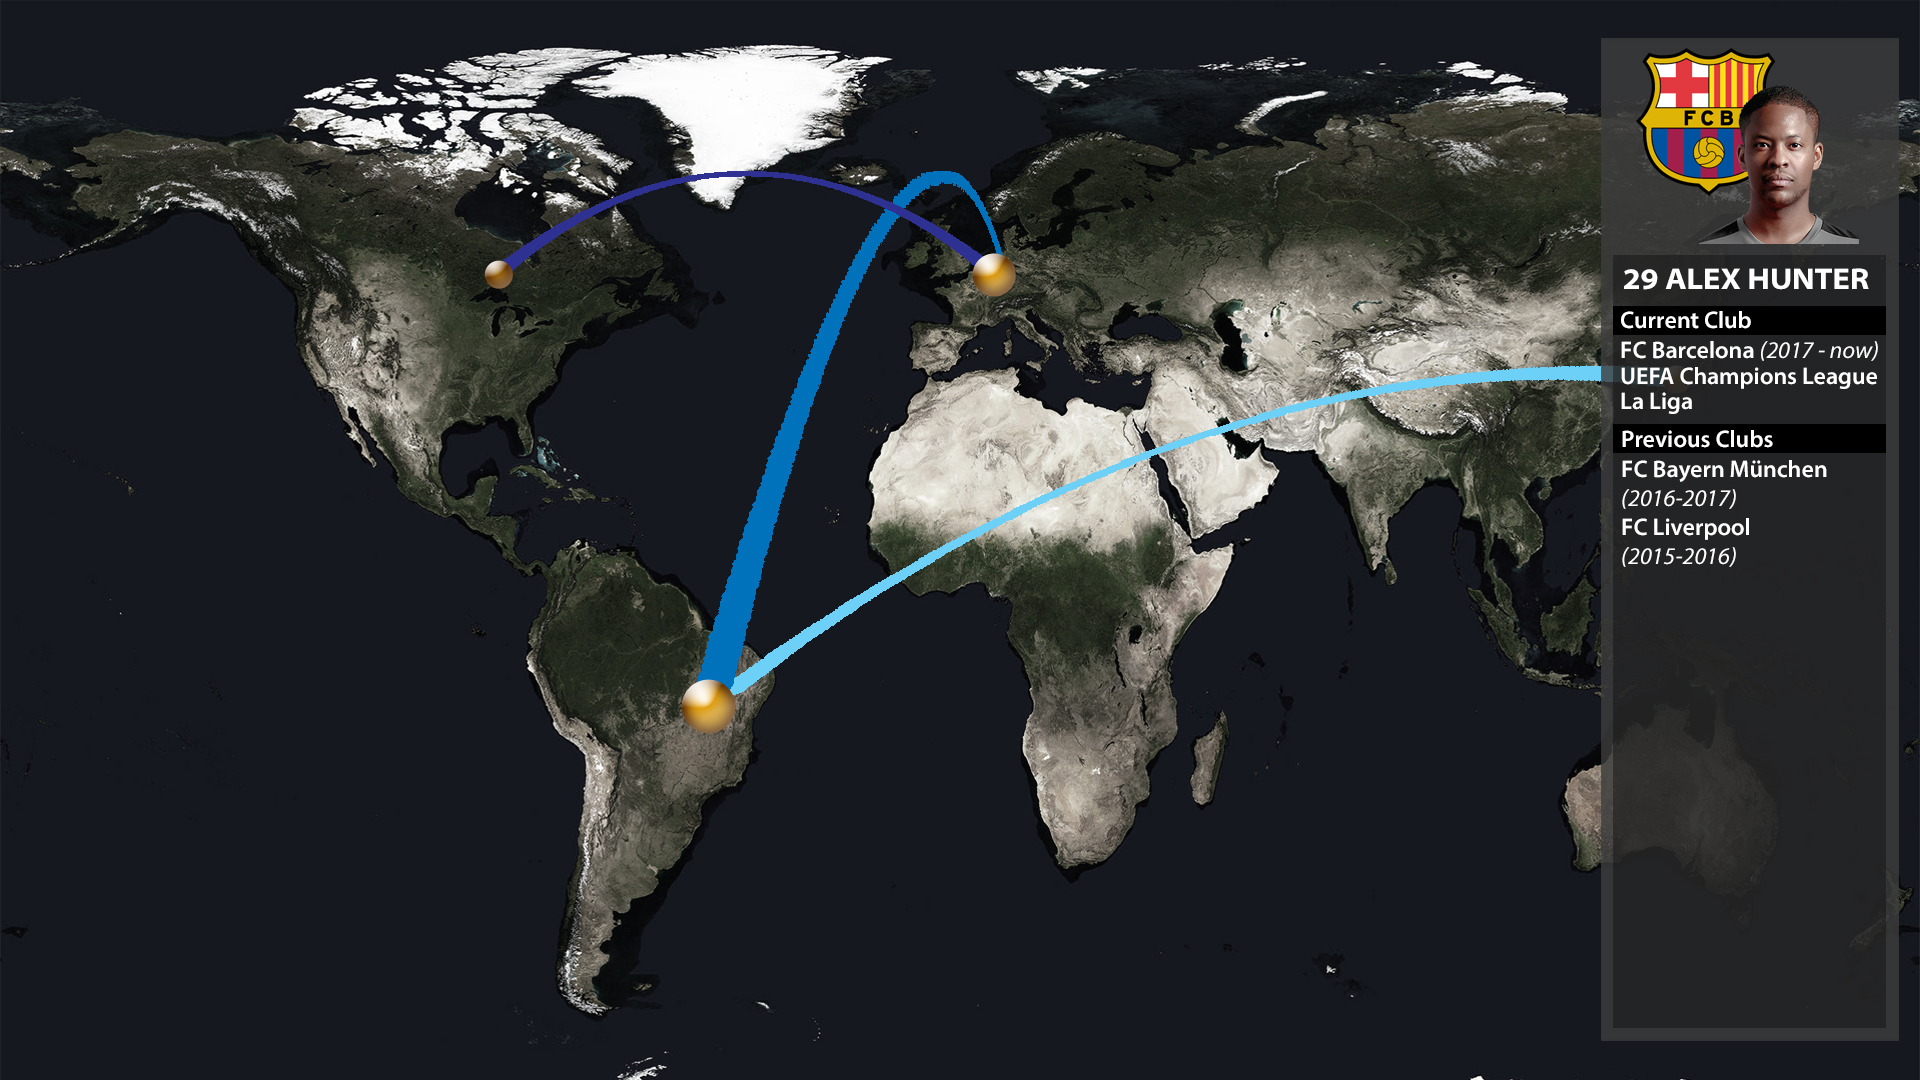
\includegraphics{Images/player_information.jpg}%
  \caption{Mockup of the map, when a player was selected.}%
\end{figure}

\begin{figure}
  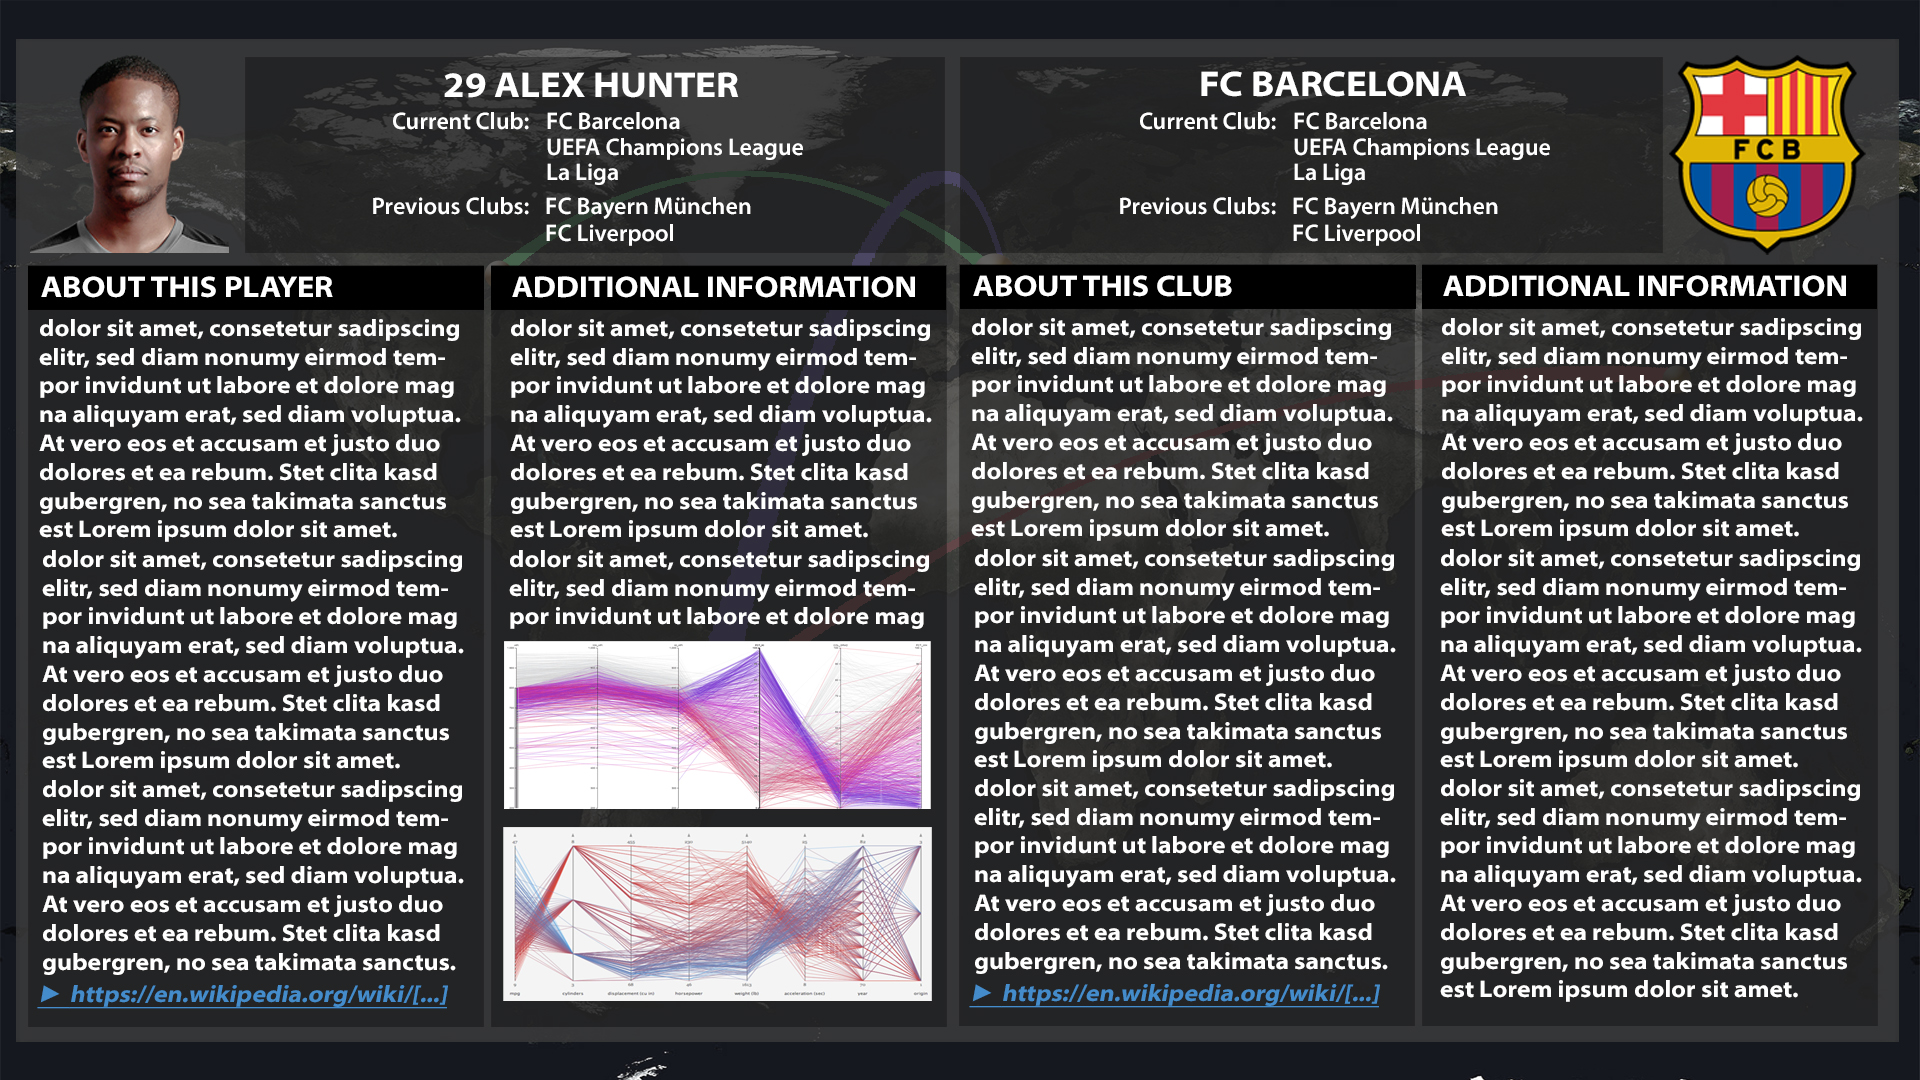
\includegraphics{Images/player_and_club_information.jpg}%
  \caption{Mockup of the visualization, when the information section of the player was extended.}%
\end{figure}

Unfortunately we had to cancel this idea due to several problems:
\begin{itemize}
	\item We could not find a database containing all the transfer data. We would have had to gather this information by crawling through the code of several websites which contain the information.
	\item Moreover the website we could crawl does not contain the transfer sum.
	\item For the players we wanted to use the FIFA database. It also containes links to pictures of the players and the logos of the clubs. But the resolution of these pictures was too low, so we would have had to replace them by higher resolution pictures.
	\item Also the encoding of the FIFA database threw up a problem with special characters in the player's names. In addition the names of the players are not normalized, so there were entries like \quo{Cristiano Ronaldo} and \quo{L. Messi}. This makes it harder to join this database with other databases.
	\item We need a database with the GPS coordinates of the stadiums of the football clubs. The database we found did only contain some countries of Europe, but there were still many important clubs missing.
\end{itemize}

\clearpage

\marginnote[1.8cm]{\quo{We don't make mistakes. We just have happy accidents.} -- \textit{Bob Ross}}
\begin{figure}
  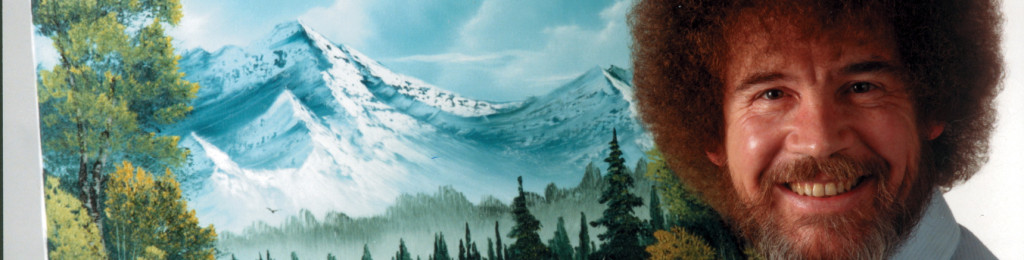
\includegraphics{Images/bob-ross1.jpg}%
  \caption{}%
\end{figure}

\section{Bob Ross}

Statistics is everywhere, even in the art! What we want to show is that the paintings can be observed in statistical manner. Inspired by instructional television program \textit{The Joy of the Painting} created and hosted by Bob Ross, we want to visualize the data about his paintings created during this 11-year television show. During 403 episodes Bob Ross painted 381 works. Each of this painting consists of distinct set of elements - \quo{happy trees}, \quo{almighty mountains}, \quo{fluffy clouds} how he used to call them. The data set that we plan to use comes from fivethirtyeight's website\cite{fivethirtyeight} and is created by exploring each episode and painting in particular. In total there are 67 keywords that describe the content of the image (trees, water, mountains, etc.). We want to use these keywords (tags) to make conclusions not just about this particular television program, but also about instructional painting. In order to explain some of the basic art concepts, what did he draw? When observing his paintings on the first sight, we can conclude that he painted mountains and water really often. But how often is it in numbers? Did the nature he was presenting change during the years (seasons), or maybe during the months (episodes)? Can we make some assumptions -- that if he draws mountains, how likely is he going to draw a house or trees? We think that the results could give us some interesting insights and conclusions about these paintings.\\
The target audience are his fans all over the world as well as people which are interested in art in general. Also people who might want to decorate their apartment with some drawings might be interested in exploring Bob Ross' paintings by selecting the elements they would like (or don't want) to see in the painting. \\

\begin{figure}
	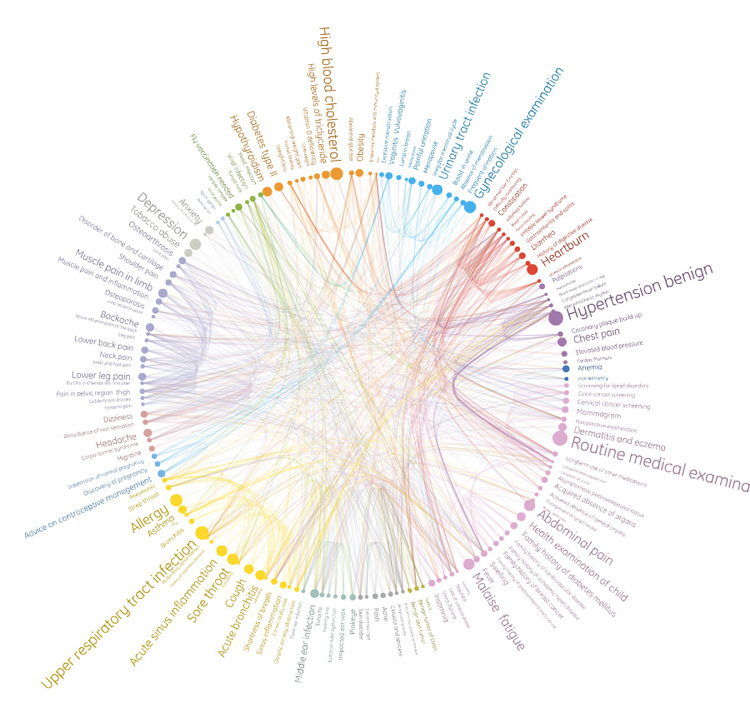
\includegraphics{Images/visualization_first_idea.jpg}
	\caption{The first idea of possible visualization. The elements are noted around the circle, connected by the lines if they appear together.}
	\label{fig:firstidea}
\end{figure}

In Figure \ref{fig:firstidea}\cite{firstidea} you can see our first idea for a visualization with the data set described above.

\newthought{Moreover} we discovered the website \href{http://www.twoinchbrush.com/}{TwoInchBrush} which contains a database of all links to pictures of Bob's paintings, the link to each episode on YouTube as well as a matrix of the used colours per painting and paintings made by guests. We contacted the owner of the website, Felix Auer, and he shared his database\cite{felixauer} with us. Thank you, Felix!\\


\chapter{Creating a Concept}

We created a draft of the concept of our visualization. Starting with collecting all the ideas we had up to this point we created an overview of the designs of the several graphs and transitions between them. 

\begin{figure}
	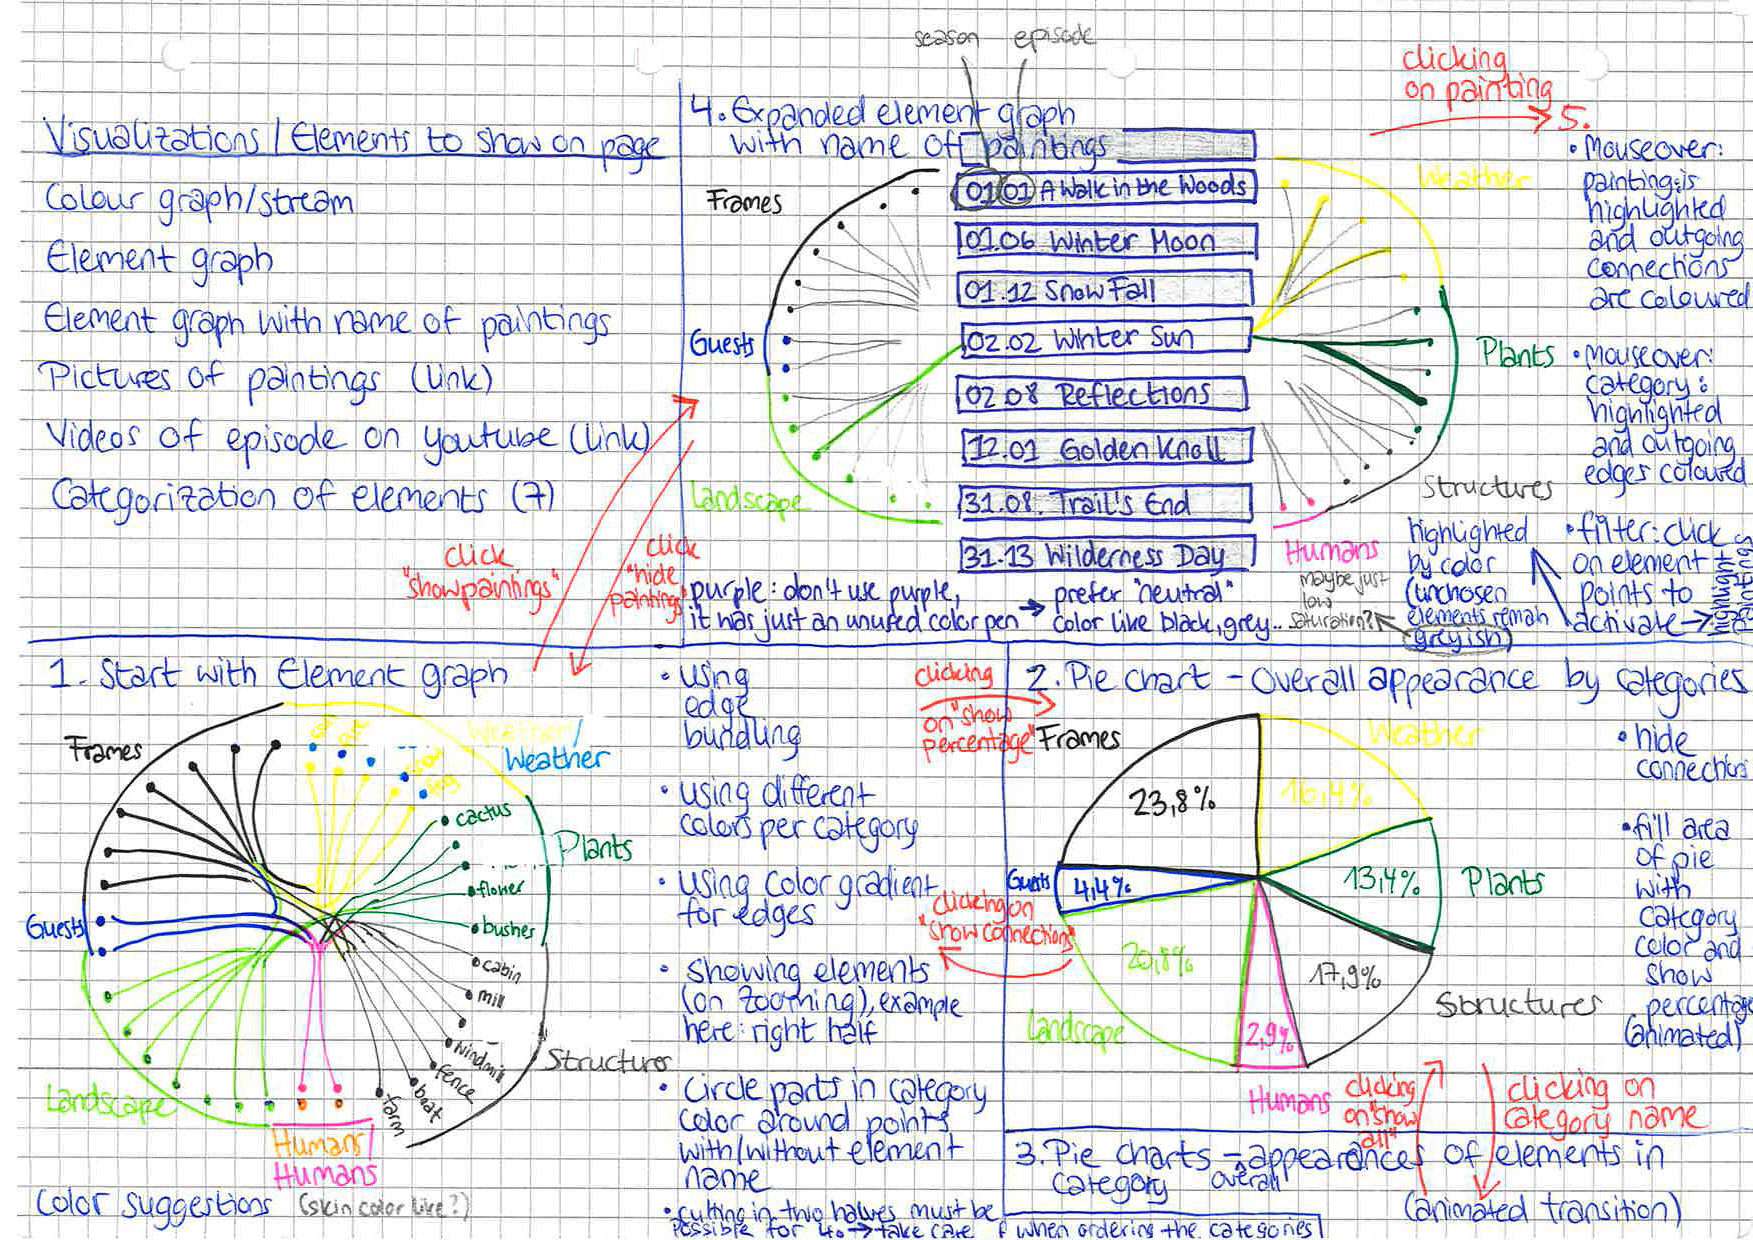
\includegraphics{Images/concept1.jpg}
	\caption{}
	\label{fig:concept1}
\end{figure}

\begin{figure}
	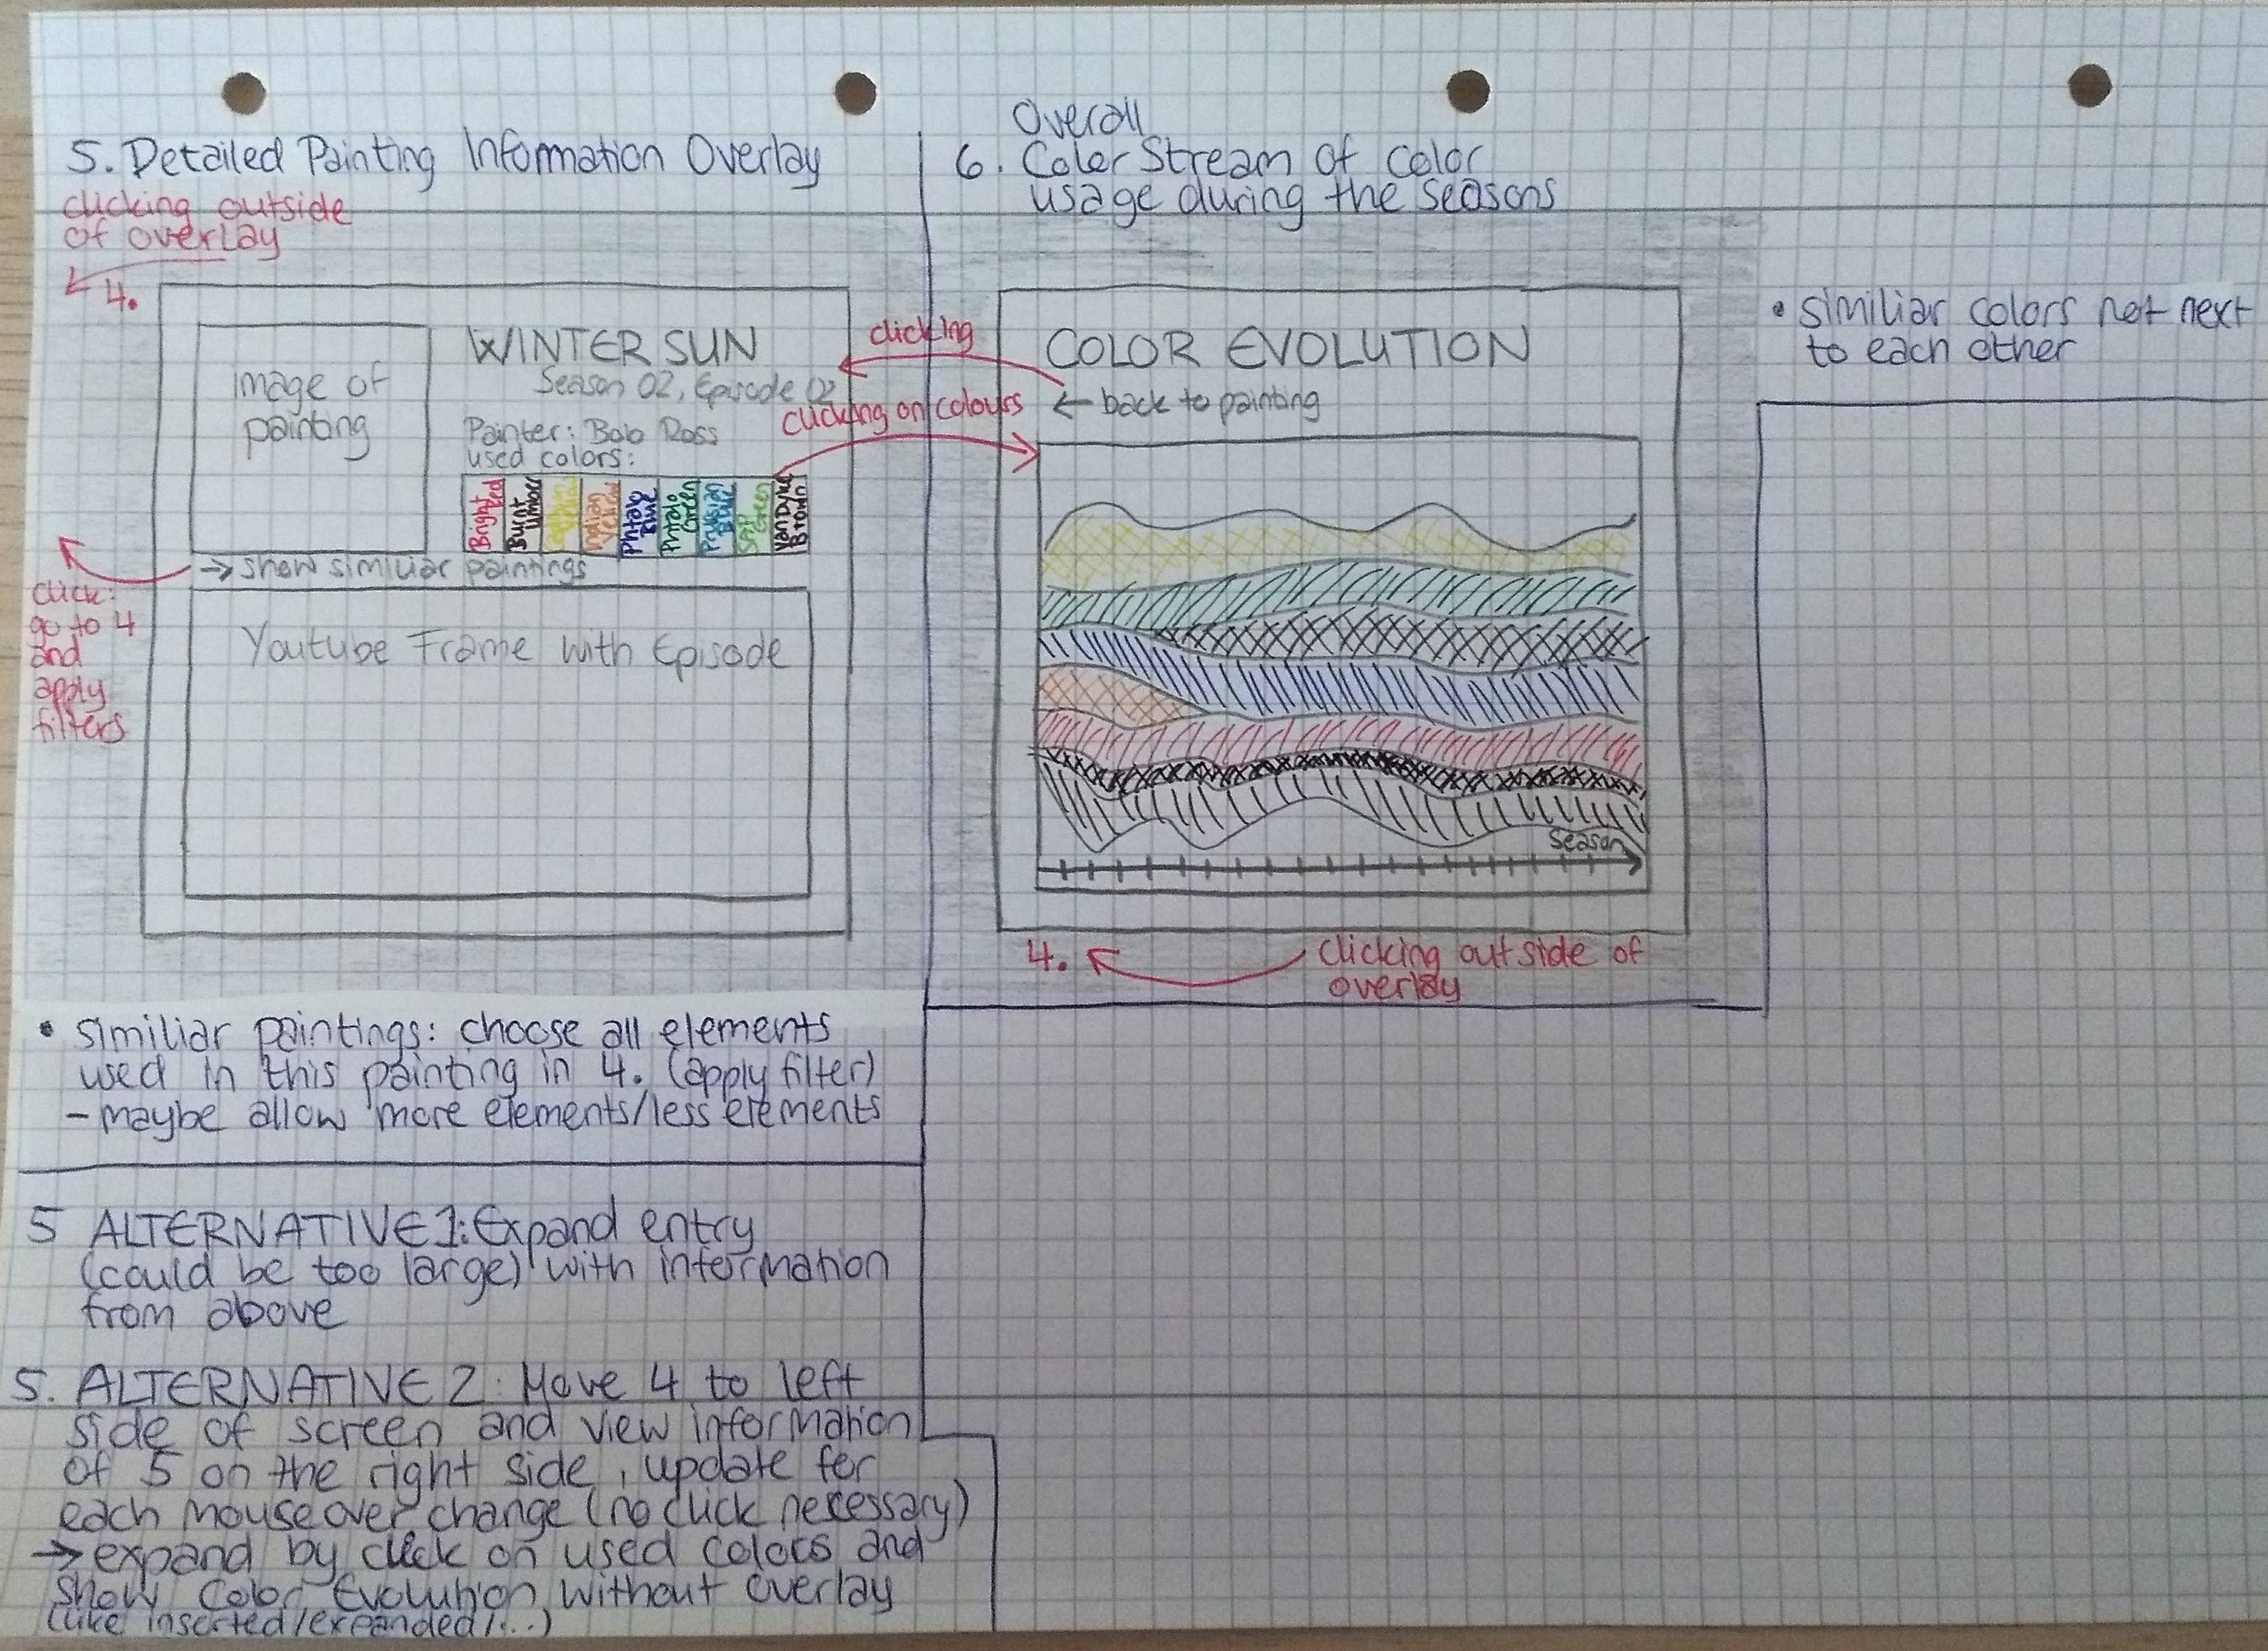
\includegraphics{Images/concept2.jpg}
	\caption{}
	\label{fig:concept2}
\end{figure}

\newthought{The basic element graph} is shown in \textbf{1} in \ref{fig:concept1}. We plan this to be our start visualization, so the first visualization that is shown to the user when he enters the website. In this graph we show all the elements and their connections to each other. That means, if there appear \quo{fog} and \quo{boat} together in a painting, there will be a connection. If these two elements appear several times together in the paintings, the connection will be stronger. We want to use a color gradient on the edges.\\
In order to make edge bundling possible, we categorized the different elements into seven categories. For each category we chose a color (and sometimes also an alternative color) that is mostly associated with the category. \\
%TODO:insert table? 
We want to draw the elements as dots in a circle and show the name of the element next to it's dot. Next to the element's names there is a circle line part in the category's color and the name of the category. 

\newthought{Pie charts} are also part of our concept. They will show the overall appearance. In \ref{fig:concept1} they are labeled with \textbf{2}. The first pie chart is shown by hiding the edges from the element graph and filling the pies with the category color and the percentage. By clicking on a category the category's pie extend to the whole circle and adds the element pies. The element pies should have a similar color to the category color, but they should all have different colors. This is referred to in \ref{fig:concept1} as \textbf{3}.

\newthought{The expanded element graph} is shown in \textbf{4} in \ref{fig:concept1}. Here we basically use the element graph of \textbf{1} and add the paintings in boxed in the middle of the splitted circle. The edges are no longer between the elements, but refer now to the appearance in the paintings. For increasing the readability of the graph, we transfer all colors to greyscale and show only the colors of the highlighted elements. Highlighted are elements by mouseover. If the mouse is over a painting, it will be highlighted for example by setting the background of it's box to white (instead of grey for the non-highlighted elements) and it's edges will be shown in the colors of the corresponding category. The same highlighting principle will be used for a mouseover on the categories respectively on the elements.\\
We can apply filters by clicking on elements (one click: add element to filter, second click: remove element from filter) and multiple elements can be chosen. By this, they will be highlighted as well as the paintings to which the filters apply.  \\

\newthought{Detailed painting informations} can be visualized as shown in \textbf{5} in \ref{fig:concept2}. This painting information section can be reached by clicking on a painting in the expanded element graph. For this visualization we drafted several alternatives which we have to try out in our implementation. The first idea is with an overlay (which is drawn in \ref{fig:concept2}). But the disadvantage of the overlay it that it does not fit in the other concepts we used. So we looked for alternatives. The second idea is to expand the painting's box in the expanded element graph and show the information in this box. But this could easily be too big for a nice visualization and destroy the expanded element graph, since it would grow very high. The third alternative is to move the expanded element graph to the left side and show the detailed painting information on the right side. This section would be updated with every change of the mouseover on a painting and by this, the user does not need to click on the painting anymore. \\

\newthought{An overall color stream} of the color usage during the seasons is also a nice way to visualize how Bob's preferences for colors might change over 31 seasons. We show how often every color was used in a season and create a graph out of this information. This section can be either shown by clicking on the used colors section in the detailed painting information (for the overlay version, as drawn in \ref{fig:concept2}) or in case of the third idea for the detailed painting information also on the right side. In order to represent the colors as exact as possible we created another database with the hexadecimal values of the used colours in the paintings. We took all hexcodes from \cite{tpark} with the exception of \quo{Black Gesso}\footnote{colour value was chosen by us}, \quo{Burnt Umber}\cite{wikiBurntUmber}, \quo{Indian Red}\cite{wikiIndianRed}, \quo{Liquid Black}\footnote{value was set by us} and \quo{Liquid Clear}\footnote{value was set by us}. 


\newthought{Concept map} - While thinking about the right way to present the elements in a graph, on the website 
 - "The Conversation" website -  we found the inspiration - concept map shown in figure x. We decided to use this idea to present elements drawn in each episode. First implementation is shown in figure x and it presents elements drawn in each episode during the first season of the TV show. Further we want to show the elements for all seasons - in total there are 31 seasons. As this probably will not fit into single graph, we will enable filtering by seasons, initally showing first few seasons. We also plan to provide filtering by different elements (for example trees, cottages, etc) or similar groups of elements (mountain landscape, winter landscape, etc).

\begin{figure}
	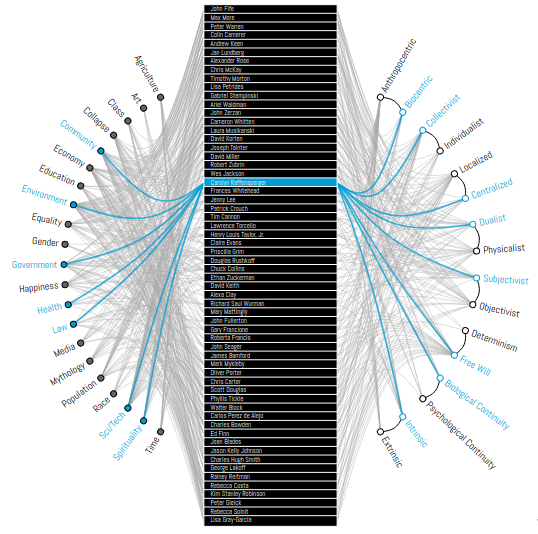
\includegraphics{Images/conceptMapIdea.png}
	\caption{Inspiration for concept map visualization - taken from website http://www.findtheconversation.com/concept-map/}
	\label{fig:concept2}
\end{figure}

\begin{figure}
	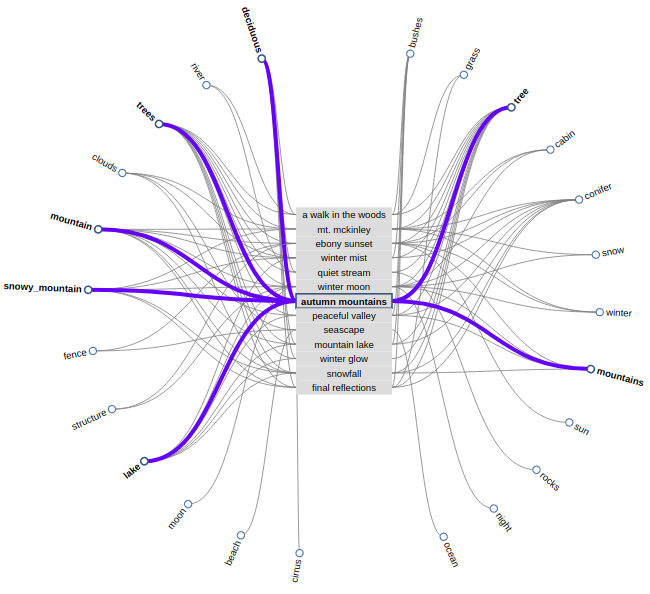
\includegraphics{Images/firstImplementation.png}
	\caption{First implementation of the concept map}
	\label{fig:concept2}
\end{figure}


%%
% The back matter contains appendices, bibliographies, indices, glossaries, etc.
\backmatter

\bibliography{bibliography}
\bibliographystyle{plainnat}


\printindex

\end{document}

